%%%%%%%%%%%%%%%%%%%%%%%%%%%%%%%%%%%%%%%%%
% Beamer Presentation
% LaTeX Template
% Version 1.0 (10/11/12)
%
% This template has been downloaded from:
% http://www.LaTeXTemplates.com
%
% License:
% CC BY-NC-SA 3.0 (http://creativecommons.org/licenses/by-nc-sa/3.0/)
%
%%%%%%%%%%%%%%%%%%%%%%%%%%%%%%%%%%%%%%%%%

%----------------------------------------------------------------------------------------
%	PACKAGES AND THEMES
%----------------------------------------------------------------------------------------

\documentclass{beamer}

\usepackage{graphicx}
%\usepackage{epstopdf}

\mode<presentation> {

% The Beamer class comes with a number of default slide themes
% which change the colors and layouts of slides. Below this is a list
% of all the themes, uncomment each in turn to see what they look like.

%\usetheme{default}
%\usetheme{AnnArbor}
%\usetheme{Antibes}
%\usetheme{Bergen}
%\usetheme{Berkeley}
%\usetheme{Berlin}
%\usetheme{Boadilla}
%\usetheme{CambridgeUS}
%\usetheme{Copenhagen}
%\usetheme{Darmstadt}
%\usetheme{Dresden}
%\usetheme{Frankfurt}
%\usetheme{Goettingen}
%\usetheme{Hannover}
%\usetheme{Ilmenau}
%\usetheme{JuanLesPins}
%\usetheme{Luebeck}
%\usetheme{Madrid}
%\usetheme{Malmoe}
%\usetheme{Marburg}
%\usetheme{Montpellier}
%\usetheme{PaloAlto}
%\usetheme{Pittsburgh}
%\usetheme{Rochester}
%\usetheme{Singapore}
%\usetheme{Szeged}
%\usetheme{Warsaw}

% As well as themes, the Beamer class has a number of color themes
% for any slide theme. Uncomment each of these in turn to see how it
% changes the colors of your current slide theme.

%\usecolortheme{albatross}
%\usecolortheme{beaver}
%\usecolortheme{beetle}
%\usecolortheme{crane}
%\usecolortheme{dolphin}
%\usecolortheme{dove}
%\usecolortheme{fly}
%\usecolortheme{lily}
%\usecolortheme{orchid}
%\usecolortheme{rose}
%\usecolortheme{seagull}
%\usecolortheme{seahorse}
%\usecolortheme{whale}
%\usecolortheme{wolverine}

%\setbeamertemplate{footline} % To remove the footer line in all slides uncomment this line
\setbeamertemplate{footline}[page number] % To replace the footer line in all slides with a simple slide count uncomment this line

\setbeamertemplate{navigation symbols}{} % To remove the navigation symbols from the bottom of all slides uncomment this line
}

\usepackage{graphicx} % Allows including images
\usepackage{booktabs} % Allows the use of \toprule, \midrule and \bottomrule in tables

%----------------------------------------------------------------------------------------
%	TITLE PAGE
%----------------------------------------------------------------------------------------

\title[Short title]{Gain of the PMT's (Fit)} % The short title appears at the bottom of every slide, the full title is only on the title page

\author{Leonid Burmistrov} % Your name
\institute[LAL, Orsay] % Your institution as it will appear on the bottom of every slide, may be shorthand to save space
{
Laboratoire de l'accelerateur lineaire \\ % Your institution for the title page
\medskip
\textit{burmist@lal.in2p3.fr} % Your email address
}
\date{16.06.2015} % Date, can be changed to a custom date

\begin{document}

\begin{frame}
\titlepage % Print the title page as the first slide
\end{frame}

\begin{frame}
\frametitle{Overview} % Table of contents slide, comment this block out to remove it
\tableofcontents % Throughout your presentation, if you choose to use \section{} and \subsection{} commands, these will automatically be printed on this slide as an overview of your presentation
\end{frame}

%----------------------------------------------------------------------------------------
%	PRESENTATION SLIDES
%----------------------------------------------------------------------------------------
\section{Fit function of the gain}
%------------------------------------------------
\begin{frame}
\frametitle{Fit function of the gain}
$\mathrm{Gain} = \frac{a^n}{(n+1)^{k*n}} * V^{k*n}$
\begin{table}
\begin{tabular}{l l l l}
\toprule
\textbf{PMT} & \textbf{n} & \textbf{a} & \textbf{k} \\
\midrule
R7378A BA1511 & 10 & 0.165784 & 0.735788\\
R7378A BA1512 & 10 & 0.132402 & 0.784792\\
R7378A BA1513 & 10 & 0.163135 & 0.742609\\
R7378A ZN2207 & 10 & 0.204533 & 0.690053\\
R762 NA0138   & 10 & 0.192359 & 0.690259\\
\bottomrule
\end{tabular}
\caption{Tables of parameters after the fit.}
\end{table}
\end{frame}
%------------------------------------------------


%------------------------------------------------
\section{R7378A BA1511}

%\input{photos.tex}
%\input{photos_v.tex}

%------------------------------------------------
\begin{frame}
\frametitle{R7378A BA1511}
%$15:34:09-09.12.2014$ 
\begin{figure}
  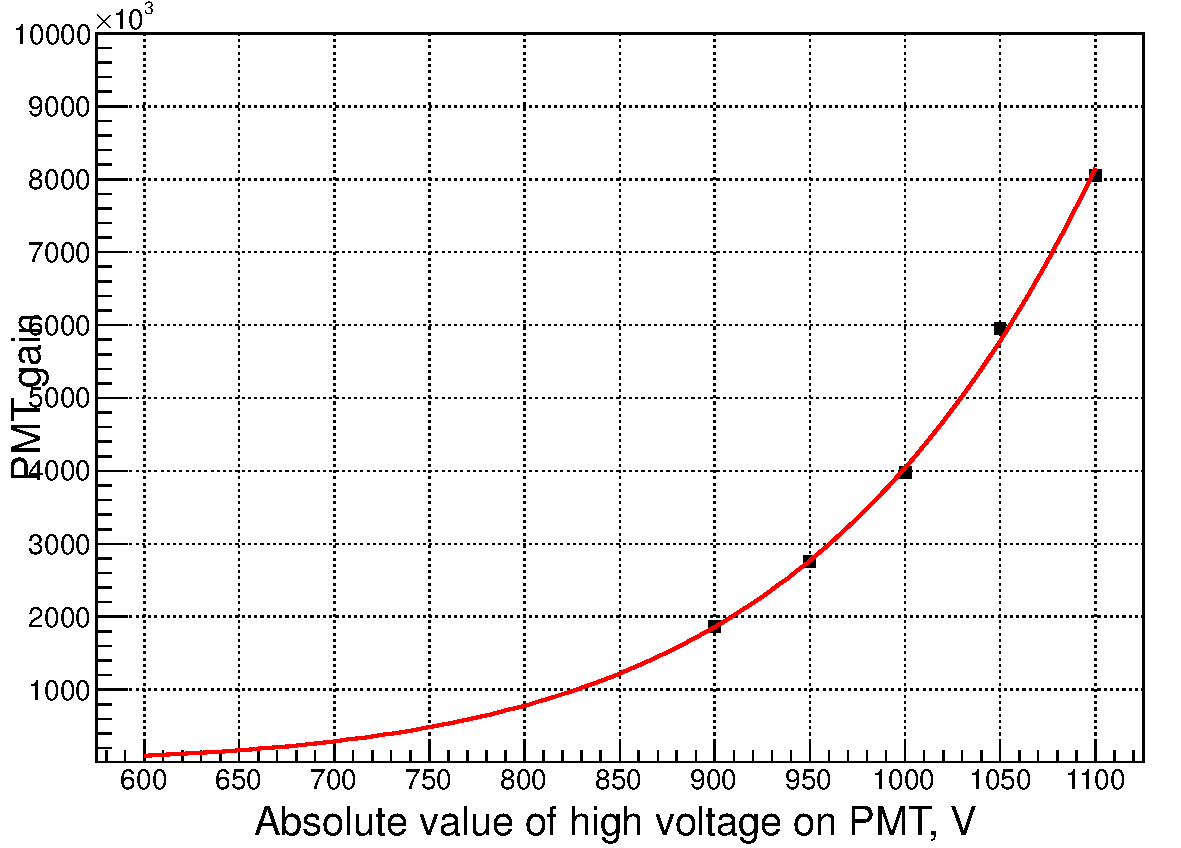
\includegraphics[width=0.95\linewidth]{./pmtGainR7378A_BA1511.pdf}
\end{figure}
\end{frame}
%------------------------------------------------
%------------------------------------------------
\begin{frame}
\frametitle{R7378A BA1511}
%$15:34:09-09.12.2014$ 
\begin{figure}
  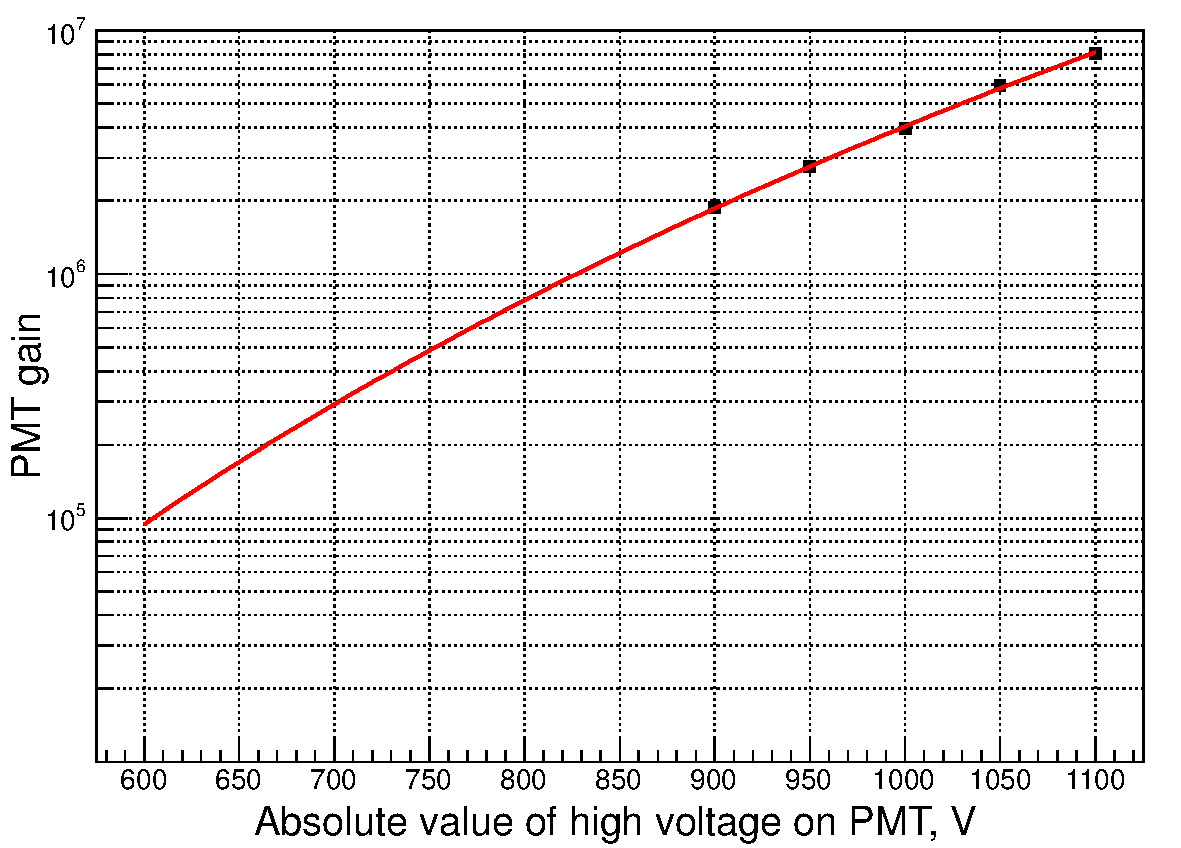
\includegraphics[width=0.95\linewidth]{./pmtGainR7378A_BA1511_log.pdf}
\end{figure}
\end{frame}
%------------------------------------------------
%------------------------------------------------
\begin{frame}
\frametitle{R7378A BA1511}
\begin{table}
\begin{tabular}{l l}
\toprule
\textbf{Hight voltage, V} & \textbf{Gain} \\
\midrule
-500 & 2.46423 * $10^4$\\
-550 &  4.96871 * $10^4$\\
-600 &  9.42513 * $10^4$\\
-650 &  1.69849 * $10^5$\\
-700 &  2.93004 * $10^5$\\
-750 &  4.86788 * $10^5$\\
-800 &  7.82657 * $10^5$\\
-850 &  1.22263 * $10^6$\\
-900 &  1.86185 * $10^6$\\
-950 &  2.77151 * $10^6$\\
-1000 &  4.04226 * $10^6$\\
-1050 &  5.78805 * $10^6$\\
-1100 &  8.15054 * $10^6$\\
\bottomrule
\end{tabular}
\caption{Table of gains}
\end{table}
\end{frame}
%------------------------------------------------



\section{R7378A BA1512}
%------------------------------------------------
\begin{frame}
\frametitle{R7378A BA1512}
\begin{figure}
  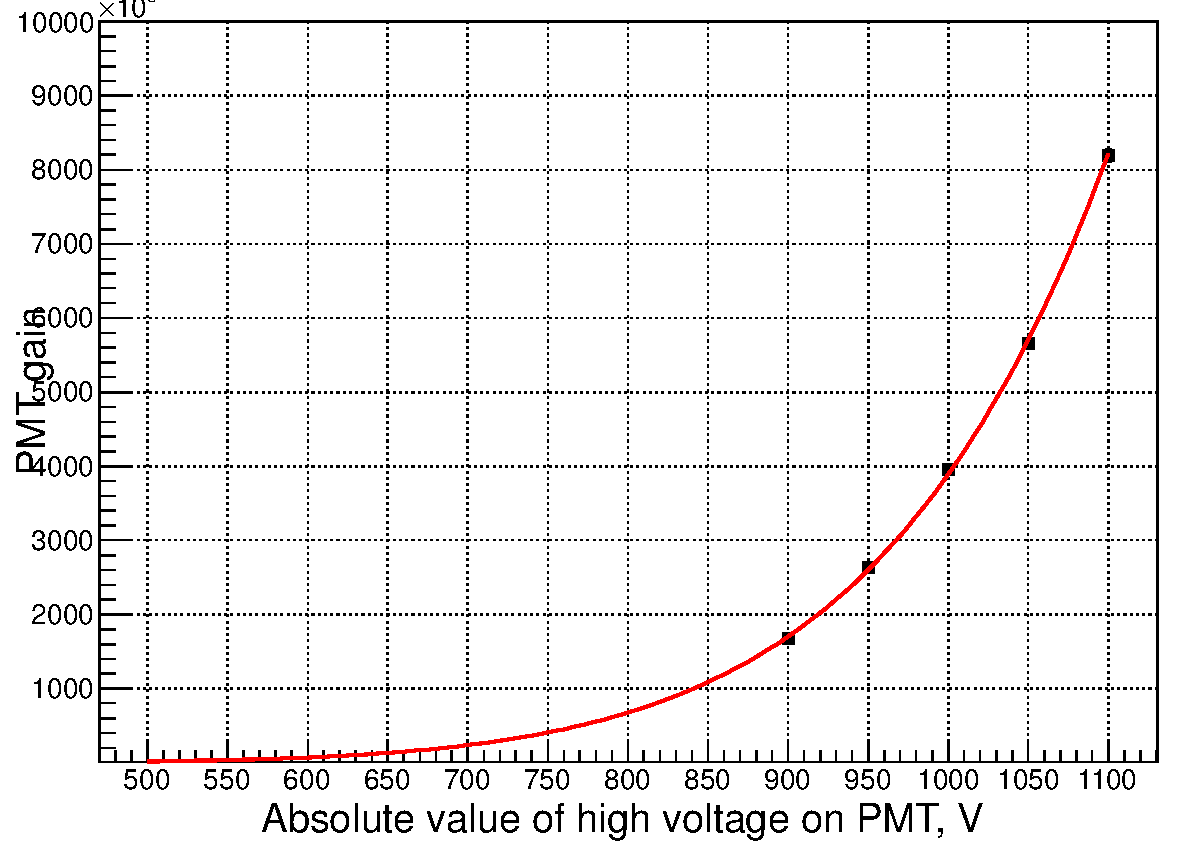
\includegraphics[width=0.95\linewidth]{./pmtGainR7378A_BA1512.pdf}
\end{figure}
\end{frame}
%------------------------------------------------
%------------------------------------------------
\begin{frame}
\frametitle{R7378A BA1512}
\begin{figure}
  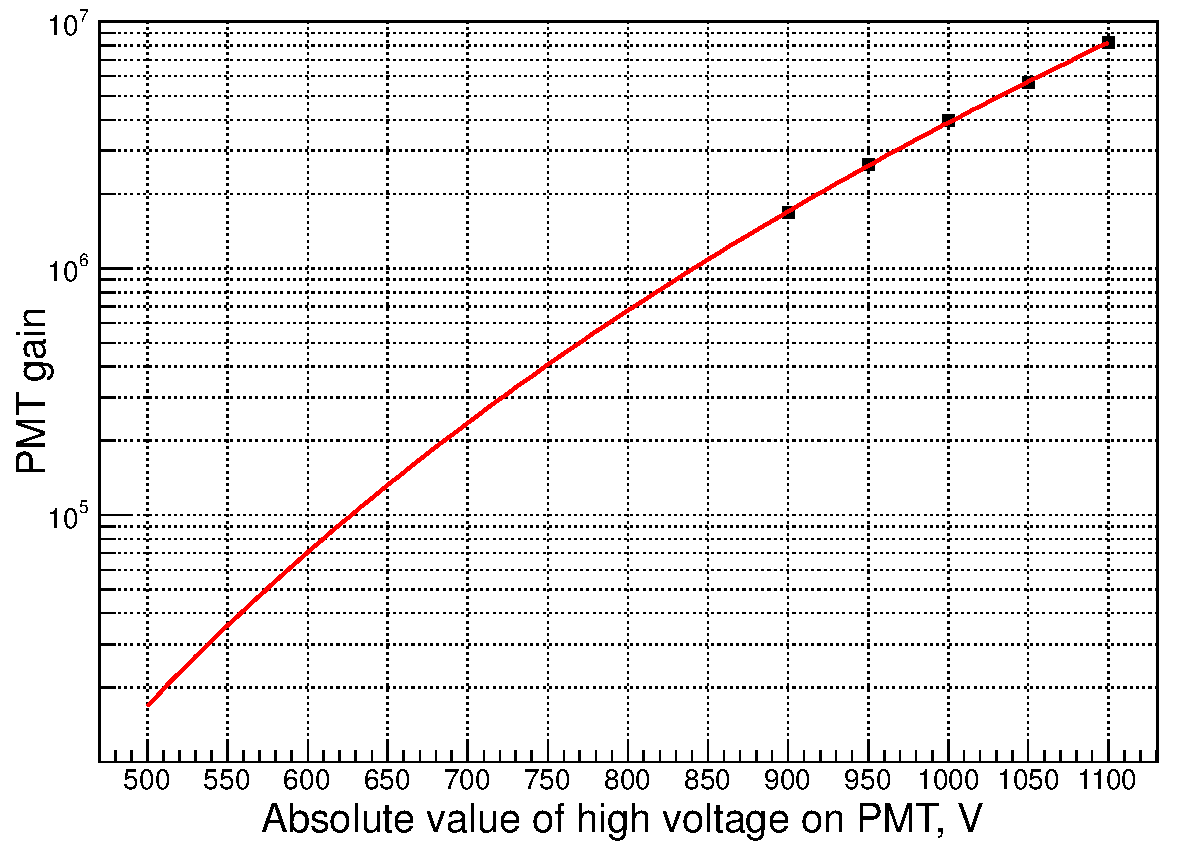
\includegraphics[width=0.95\linewidth]{./pmtGainR7378A_BA1512_log.pdf}
\end{figure}
\end{frame}
%------------------------------------------------
%------------------------------------------------
\begin{frame}
\frametitle{R7378A BA1512}
\begin{table}
\begin{tabular}{l l}
\toprule
\textbf{Hight voltage, V} & \textbf{Gain} \\
\midrule
-500 &  1.68842 * $10^4$\\
-550 &  3.56719 * $10^4$\\
-600 &  7.06135 * $10^4$\\
-650 &  1.32342 * $10^5$\\
-700 &  2.36745 * $10^5$\\
-750 &  4.06846 * $10^5$\\
-800 &  6.75145 * $10^5$\\
-850 &  1.08649 * $10^6$\\
-900 &  1.70152 * $10^6$\\
-950 &  2.60085 * $10^6$\\
-1000 &  3.88990 * $10^6$\\
-1050 &  5.70467 * $10^6$\\
-1100 &  8.21837 * $10^6$\\
\bottomrule
\end{tabular}
\caption{Table of gains}
\end{table}
\end{frame}
%------------------------------------------------

\section{R7378A BA1513}
%------------------------------------------------
\begin{frame}
\frametitle{R7378A BA1513}
\begin{figure}
  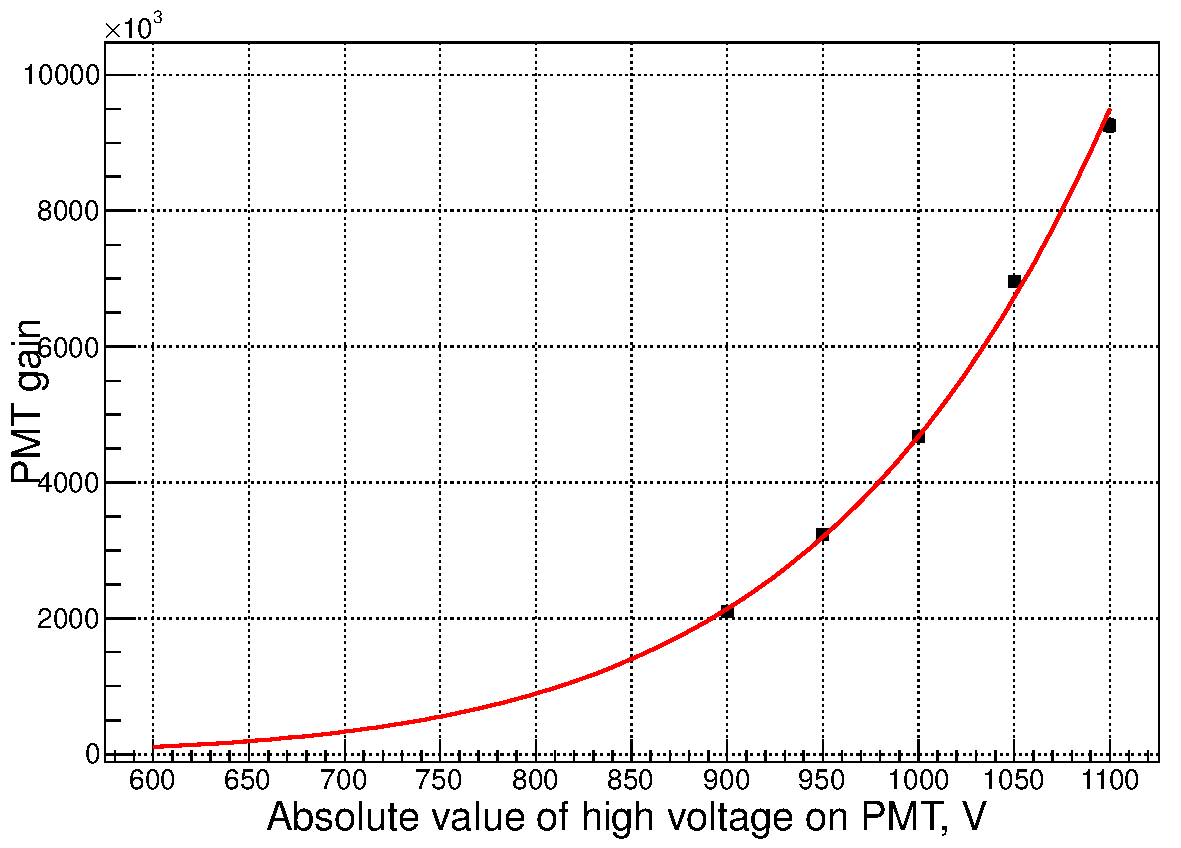
\includegraphics[width=0.95\linewidth]{./pmtGainR7378A_BA1513.pdf}
\end{figure}
\end{frame}
%------------------------------------------------
%------------------------------------------------
\begin{frame}
\frametitle{R7378A BA1513}
\begin{figure}
  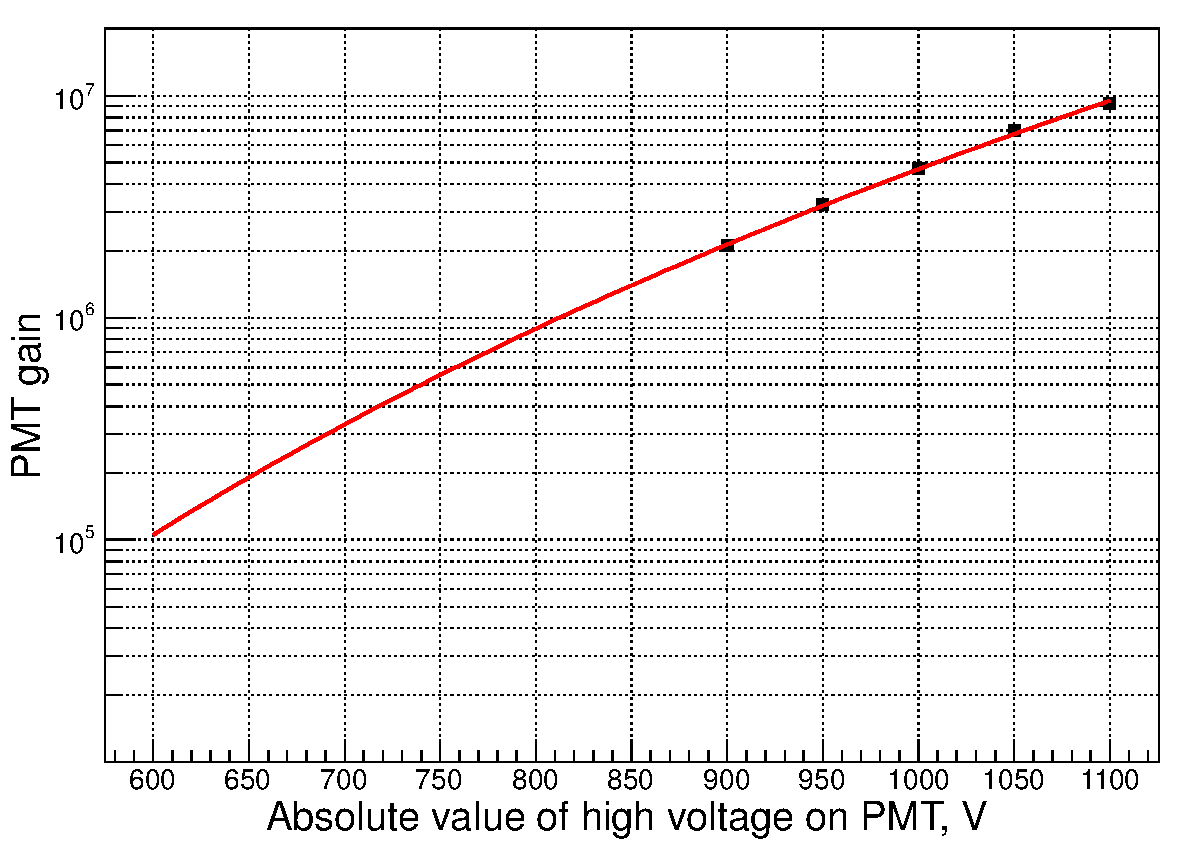
\includegraphics[width=0.95\linewidth]{./pmtGainR7378A_BA1513_log.pdf}
\end{figure}
\end{frame}
%------------------------------------------------
%------------------------------------------------
\begin{frame}
\frametitle{R7378A BA1513}
\begin{table}
\begin{tabular}{l l}
\toprule
\textbf{Hight voltage, V} & \textbf{Gain} \\
\midrule
-500  &  2.72138 * $10^4$\\
-550  &  5.52301 * $10^4$\\
-600  &  1.05389 * $10^5$\\
-650  &  1.90960 * $10^5$\\
-700  &  3.31093 * $10^5$\\
-750  &  5.52662 * $10^5$\\
-800  &  8.92490 * $10^5$\\
-850  &  1.39999 * $10^6$\\
-900  &  2.14026 * $10^6$\\
-950  &  3.19771 * $10^6$\\
-1000 &  4.68021 * $10^6$\\
-1050 &  6.72387 * $10^6$\\
-1100 &  9.49842 * $10^6$\\
\bottomrule
\end{tabular}
\caption{Table of gains}
\end{table}
\end{frame}
%------------------------------------------------



\section{R7378A ZN2207}
%------------------------------------------------
\begin{frame}
\frametitle{R7378A ZN2207}
\begin{figure}
  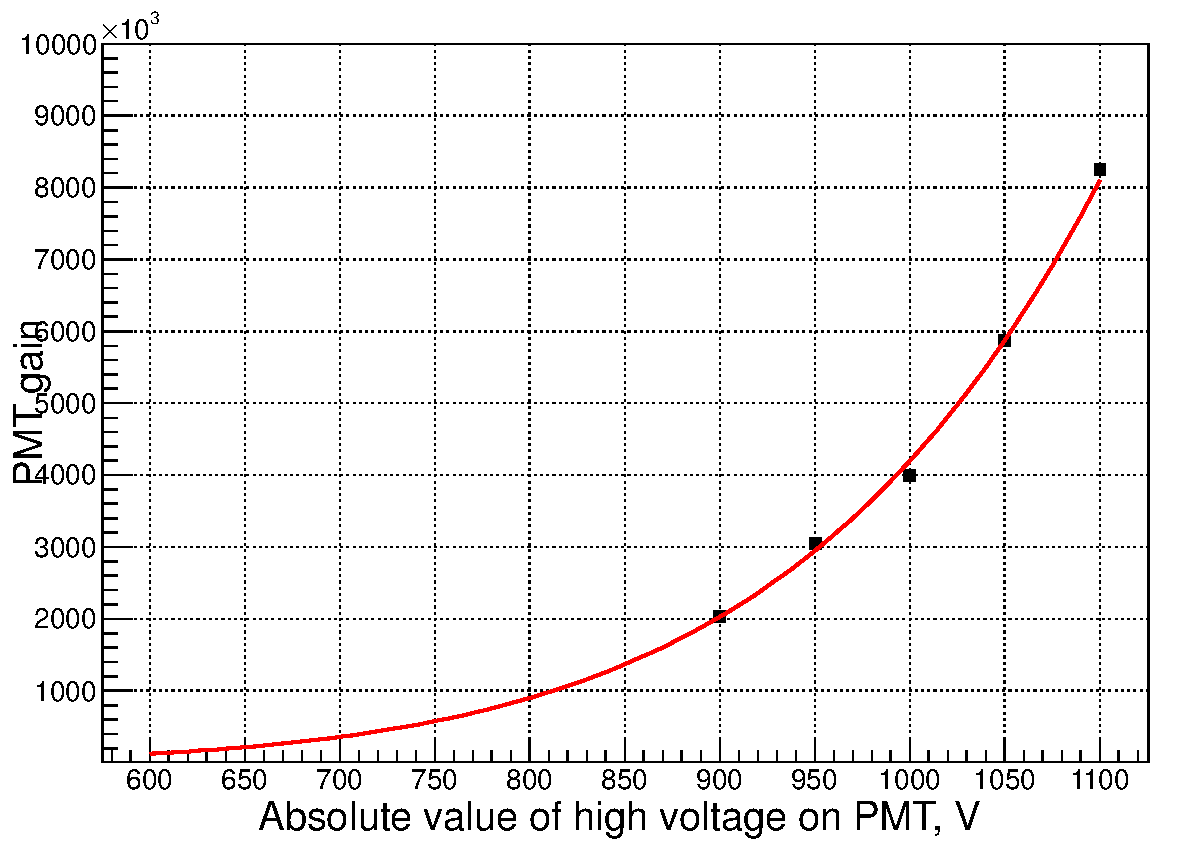
\includegraphics[width=0.95\linewidth]{./pmtGainR7378A_ZN2207.pdf}
\end{figure}
\end{frame}
%------------------------------------------------
%------------------------------------------------
\begin{frame}
\frametitle{R7378A ZN2207}
\begin{figure}
  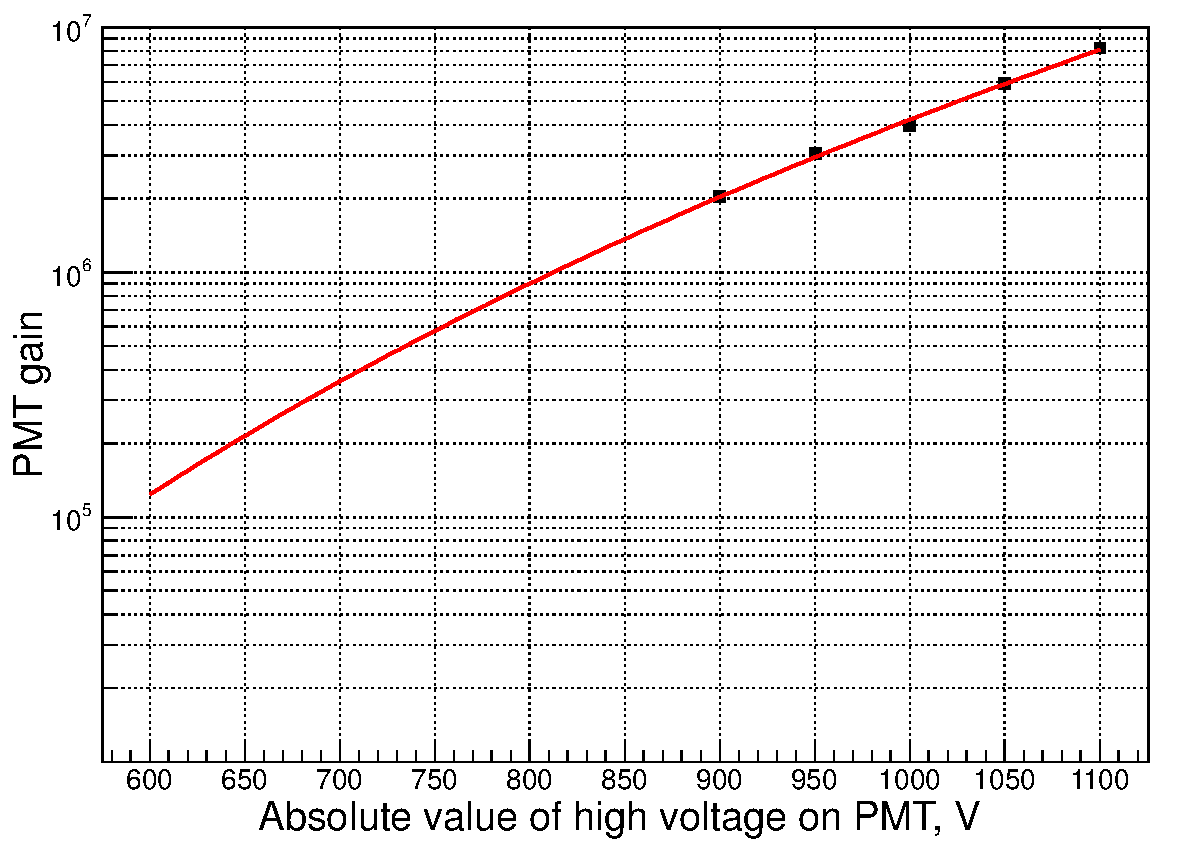
\includegraphics[width=0.95\linewidth]{./pmtGainR7378A_ZN2207_log.pdf}
\end{figure}
\end{frame}
%------------------------------------------------
%------------------------------------------------
\begin{frame}
\frametitle{R7378A ZN2207}
\begin{table}
\begin{tabular}{l l}
\toprule
\textbf{Hight voltage, V} & \textbf{Gain} \\
\midrule
-500  &  3.51395 * $10^4$\\
-550  &  6.78309 * $10^4$\\
-600  &  1.23648 * $10^5$\\
-650  &  2.14815 * $10^5$\\
-700  &  3.58226 * $10^5$\\
-750  &  5.76659 * $10^5$\\
-800  &  9.00185 * $10^5$\\
-850  &  1.36778 * $10^6$\\
-900  &  2.02914 * $10^6$\\
-950  &  2.94675 * $10^6$\\
-1000 &  4.19819 * $10^6$\\
-1050 &  5.87868 * $10^6$\\
-1100 &  8.10390 * $10^6$\\
\bottomrule
\end{tabular}
\caption{Table of gains}
\end{table}
\end{frame}
%------------------------------------------------





\section{R762 NA0138 (typical gain)}
%------------------------------------------------
\begin{frame}
\frametitle{R762 NA0138 (typical gain)}
\begin{figure}
  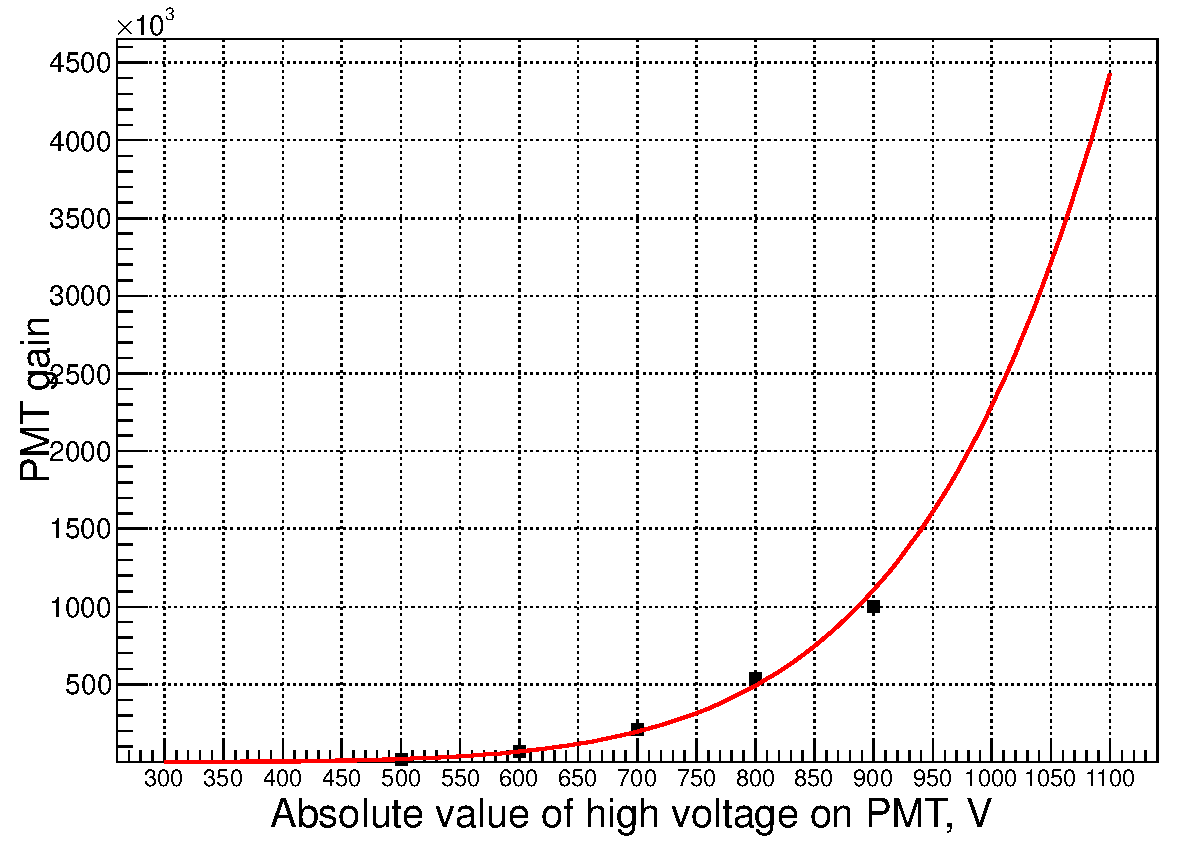
\includegraphics[width=0.95\linewidth]{./pmtTypicalGainR762_NA0138.pdf}
\end{figure}
\end{frame}
%------------------------------------------------
%------------------------------------------------
\begin{frame}
\frametitle{R762 NA0138 (typical gain)}
\begin{figure}
    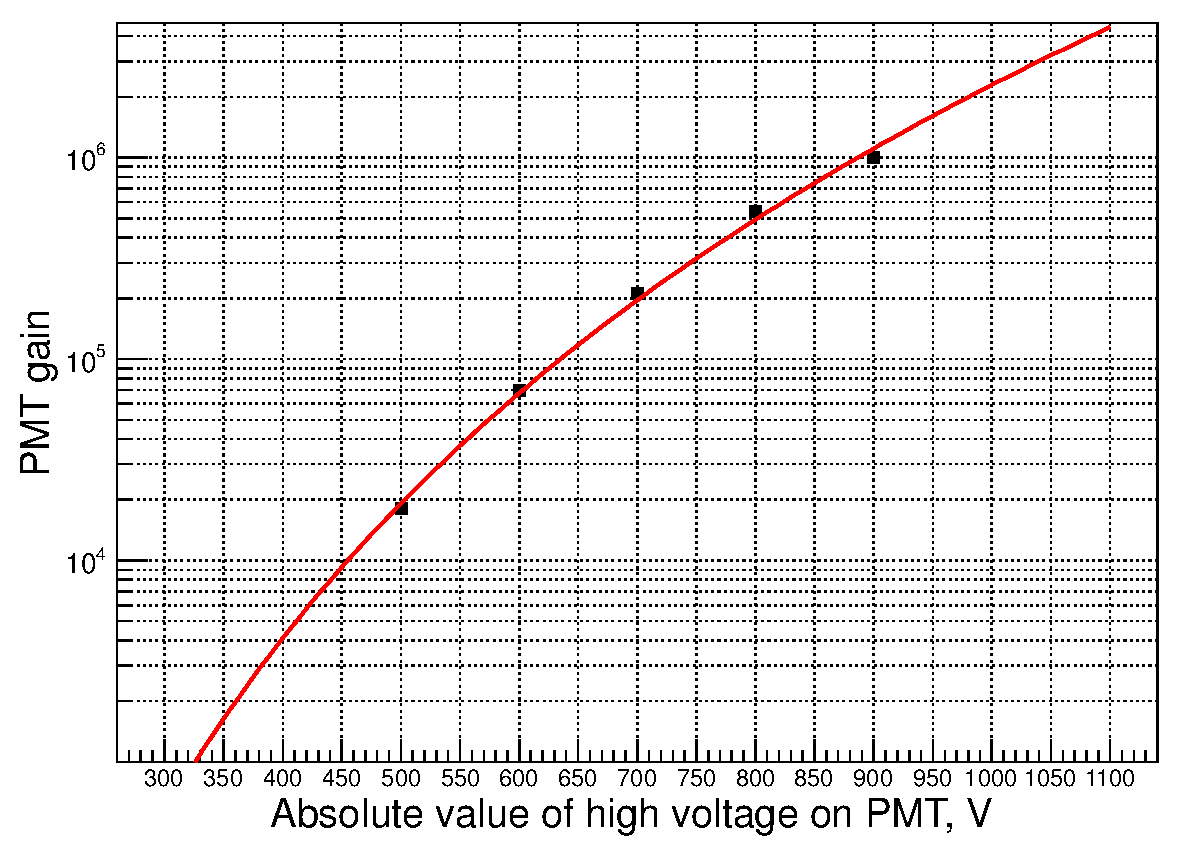
\includegraphics[width=0.95\linewidth]{./pmtTypicalGainR762_NA0138_log.pdf}
\end{figure}
\end{frame}
%------------------------------------------------
%------------------------------------------------
\begin{frame}
\frametitle{R762 NA0138 (typical gain)}
\begin{table}
\begin{tabular}{l l}
\toprule
\textbf{Hight voltage, V} & \textbf{Gain} \\
\midrule
-400  &  4.10934 * $10^3$\\
-450  &  9.26524 * $10^3$\\
-500  &  1.91735 * $10^4$\\
-550  &  3.70185 * $10^4$\\
-600  &  6.74928 * $10^4$\\
-650  &  1.17275 * $10^5$\\
-700  &  1.95598 * $10^5$\\
-750  &  3.14911 * $10^5$\\
-800  &  4.91653 * $10^5$\\
-850  &  7.47130 * $10^5$\\
-900  &  1.10852 * $10^6$\\
-950  &  1.60999 * $10^6$\\
-1000 &  2.29397 * $10^6$\\
-1050 &  3.21255 * $10^6$\\
-1100 &  4.42899 * $10^6$\\
\bottomrule
\end{tabular}
\end{table}
\end{frame}
%------------------------------------------------

%------------------------------------------------

\begin{frame}
\Huge{\centerline{The End}}
\end{frame}

%----------------------------------------------------------------------------------------

\end{document} 
